% Chapter 2

\chapter{A Mutual Information-based Multiple Level Discretization Network Inference from Time-series Gene Expression Profiles} % Main chapter title

\label{Chapter2} % For referencing the chapter elsewhere, use \ref{Chapter1} 

%----------------------------------------------------------------------------------------

% Define some commands to keep the formatting separated from the content 
%\newcommand{\keyword}[1]{\textbf{#1}}
%\newcommand{\tabhead}[1]{\textbf{#1}}
%\newcommand{\code}[1]{\texttt{#1}}
%\newcommand{\file}[1]{\texttt{\bfseries#1}}
%\newcommand{\option}[1]{\texttt{\itshape#1}}

%----------------------------------------------------------------------------------------

\section{Abstract}
Inferring GRNs from time-series gene expression data remains a fundamental yet challenging problem in systems biology because it enables researchers to decipher the dynamic transcriptional programs that govern cellular behavior. Information theoretic approaches, particularly those based on mutual information (MI), have been widely used due to their ability to capture nonlinear and nonparametric dependencies among genes. However, the performance of MI-based inference often suffers from inappropriate discretization of continuous expression profiles, which can introduce information loss, obscure temporal patterns, and reduce the accuracy of reconstructed regulatory interactions.

To overcome these limitations, this study introduces a Mutual Information based on Multi-Level Discretization Network Inference (MIDNI) framework tailored for GRN inference from temporal gene expression data. The framework adaptively partitions expression values into informative levels by jointly considering local statistical variance and global entropy characteristics. This dual criteria strategy preserves essential temporal dynamics while mitigating the influence of stochastic noise, thereby yielding more reliable MI estimates and improving the detection of regulatory relationships.

The proposed method was rigorously evaluated using benchmark datasets generated by GeneNetWeaver (GNW) and employed in the DREAM network inference challenges, which represent widely accepted standards for assessing GRN reconstruction algorithms. Comparative experiments demonstrated that MIDNI consistently outperforms traditional discretization techniques such as equal-width and equal frequency binning. Notably, improvements were observed across key evaluation metrics, including precision and recall.

Overall, the results indicate that MIDNI provides a principled and robust discretization strategy for MI-based GRN inference from time-series gene expression data. Its resilience to noise, sampling variability, and limited sample sizes makes it particularly suitable for realistic biological datasets. By enhancing the quality of MI estimation and preserving critical temporal information, the proposed framework substantially advances the accuracy and interpretability of dynamic GRN reconstruction.

%----------------------------------------------------------------------------------------

\section{Introduction}\label{chapter2_introduction}

\subsection{Motivation}

GRNs represent the intricate set of interactions among genes that collectively govern transcriptional activity, thereby orchestrating the functional behavior of organisms. Deciphering the structure and dynamics of GRNs is crucial for understanding both normal cellular processes and the molecular basis of diseases. Despite significant progress in systems biology, accurately reconstructing GRNs remains an enduring challenge due to the complexity, noise, and high dimensionality of genomic data.

The rapid advancement of high-throughput measurement technologies has enabled the collection of large scale gene expression data under diverse experimental conditions, including time-series and steady state profiles. This progress has motivated the development of numerous computational frameworks that employ statistical inference and machine learning techniques to reverse engineer GRNs. Although these approaches have substantially improved computational efficiency, alternative strategies for representing gene expression data continue to play an essential role in further accelerating inference procedures and enhancing reconstruction accuracy. Among the various representation schemes, binary encoding has been particularly influential and widely adopted, forming the basis of Boolean network models. Several established GRN inference methods, such as Best-Fit \parencite{Lahdesmaki2003} and the Mutual information-based Boolean network inference (MIBNI) methods \parencite{Barman2017}, rely on this binary abstraction to reduce computational complexity while capturing key regulatory relationships.

While these existing methods have reached a certain level of maturity and have demonstrated promising results, their performance on real biological datasets often remains suboptimal. Limitations arise from factors such as measurement noise, biological variability, simplified data representation, and the intrinsic difficulty of modeling nonlinear regulatory interactions. These shortcomings underscore the need for continued methodological advancements that improve both inference accuracy and computational scalability.

The motivation for this chapter arises from these persistent challenges and the necessity to explore improved computational strategies for GRN reconstruction. By addressing the limitations of current approaches and proposing refined methodologies, this work aims to contribute to more accurate, efficient, and biologically relevant inference of gene regulatory networks.

\subsection{Problem Statement}
GRNs has traditionally relied on Boolean network models, in which gene expression values are discretized into two states. In this representation, the value \enquote{1} denotes an active or upregulated gene state, whereas \enquote{0} corresponds to an inactive or downregulated state. Boolean models are appealing due to their conceptual simplicity, computational efficiency, and their ability to capture essential aspects of gene–gene interactions within dynamic systems. However, the coarse nature of binary discretization inevitably leads to substantial information loss, and this limitation can significantly degrade inference performance in cases where the underlying biological signals exhibit more nuanced expression patterns.

To alleviate this problem, several studies \parencite{Madeira2005, Gallo2013, Ji2004} have introduced higher order discretization schemes in which gene expression levels are mapped to three states, typically represented as \enquote{1}, \enquote{0}, and \enquote{-1}, corresponding to \enquote{upregulated}, \enquote{no-change}, and \enquote{downregulated}. Although this ternary representation has shown improvements over strict binary discretization, many existing methods adopt a fixed three-level scheme for all genes, regardless of their expression characteristics. This uniform approach is often suboptimal, as different genes may exhibit distinct variability and dynamic ranges, making some better suited for binary discretization while others require a more nuanced, multi-level representation.

Motivated by the need to reduce information loss while maintaining the computational strengths of Boolean-inspired models, we propose a novel framework termed Mutual Information based Multi-Level Discretization Network Inference (MIDNI). This method adaptively assigns each gene to either binary or ternary discretization based on the statistical distribution of its expression profile. By tailoring the discretization level to individual gene behavior, the framework aims to preserve informative expression dynamics and improve the reliability of mutual information estimation during network reconstruction.

In this chapter, we describe the criteria used to determine the appropriate discretization level for each gene, outline the design and implementation of the MIDNI inference algorithm, and present comparative results demonstrating its performance advantages. Through this adaptive discretization strategy, the proposed approach seeks to balance interpretability, computational efficiency, and accuracy in GRN inference from gene expression data.

\subsection{Existing Solutions}
 
Numerous efforts have been made by both industry practitioners and academic researchers to address the challenging problem of inferring GRNs. These efforts have led to the development of a variety of computational approaches, which can broadly be categorized into data-driven methods, correlation-based techniques, mutual information-based frameworks, tree-based algorithms, and Bayesian inference models. A critical step in these approaches is the accurate identification of regulatory genes within the input network, as this information is essential for a comprehensive understanding of the underlying biological system. This area has attracted considerable attention in the research community, resulting in numerous studies that propose novel strategies for network reconstruction. From these advances, more efficient and flexible methods have emerged, demonstrating improved performance, particularly when applied to large-scale gene expression datasets.
\subsection{Research Objectives}

Using representative or transformed data for GRN inference often yields results that are comparable to those obtained from raw expression profiles, while substantially accelerating the computational process. Among clustering techniques used for data representation, the K-means algorithm is particularly popular due to its simplicity, efficiency, and stable clustering behavior. However, determining the optimal number of clusters remains a difficult and unresolved problem. Many studies rely on the Elbow method, which requires visually inspecting the Elbow plot to decide the appropriate cluster number. This approach is inherently subjective, and in many cases the decision is ambiguous, making it challenging to reliably identify the optimal clustering configuration.

Therefore, the first objective of this study is to identify a quantitative and biologically meaningful metric that can automatically determine the suitable number of clusters to be used as a parameter for the K-means algorithm. Once an appropriate data representation is established, attention is directed toward the inference stage. The goal is to develop an algorithm capable of identifying regulatory candidates for each target gene by considering the collective interactions among all genes in the network, rather than evaluating only pairwise dependencies between a target gene and individual regulators as done in many previous approaches. This more holistic perspective is essential because it better reflects the complexity and combinatorial nature of real biological regulatory systems.

Finally, the proposed algorithm must demonstrate not only strong performance in structural accuracy correctly identifying regulatory edges but also robust performance in reproducing the dynamic behavior of the network. This capability is rarely assessed in existing methods, yet it is crucial because different regulatory structures can sometimes generate similar temporal dynamics. In summary, the algorithm aims to achieve both accurate structural prediction and faithful reconstruction of gene interaction dynamics, thereby providing a more comprehensive understanding of gene regulatory mechanisms.
%----------------------------------------------------------------------------------------
\subsection{Outline of the Chapter}
This chapter is organized into five sections, each addressing a different component of the research. 

Section ~\ref{chapter2_introduction}, which is the present section, introduces the overall subject of the chapter. It defines the research problem, outlines the motivation for addressing it, and highlights current approaches while identifying the gaps that motivate this study.

Section ~\ref{chapter2_backgound} provides an overview and critical review of the literature related to GRN inference. This section discusses a range of existing computational methodologies, examines their underlying principles, and summarizes previous work relevant to the reconstruction of gene regulatory networks.

Section ~\ref{chapter2_methodology} describes the proposed methodology, referred to as MIDNI. It provides a detailed explanation of the data representation strategy, the adaptive discretization process, and the procedure used to determine a set of candidate regulatory genes for each target gene in the network.

Section ~\ref{chapter2_result} presents the experimental setup, evaluation procedures, and results obtained from applying the proposed method. This section compares the performance of the MIDNI framework with existing baseline approaches, assessing both structural accuracy and the ability to reproduce network dynamics.

Section ~\ref{chapter2_conclusion} concludes the thesis by summarizing the major contributions and findings of the research. It also discusses limitations and outlines directions for future work aimed at further improving GRN inference methodologies.

\section{Backgrounds}\label{chapter2_backgound}

\subsection{Overview of gene regulatory network inference}

A GRN is a system of molecular regulators that interact with one another and with various cellular components to control the expression levels of mRNA and proteins, which ultimately determine cellular function. GRNs are also fundamental to morphogenesis, the process by which organisms develop their structural form, making them central to the field of evolutionary developmental biology.

Inferring GRNs provides essential insights into the behavior of biological systems. By understanding these regulatory interactions, researchers can identify disease-specific mechanisms, which can subsequently guide the development of targeted therapeutic interventions. Thus, reconstructing gene regulatory networks is a critical step toward unraveling complex biological processes and advancing medical research.

GRNs serve as powerful abstractions that capture the organizational principles of genetic regulation. Following the emergence of high-throughput measurement technologies in the late 1990s, the reconstruction of GRN structures became a major computational challenge within systems biology. Although substantial methodological progress has been achieved over the past two decades, the problem remains far from completely solved, with significant room for improvement in accuracy, scalability, and robustness. Consequently, the scientific community continues to develop more effective computational strategies to address these limitations.

In this study, we introduce a new approach for GRN inference using time-series gene expression data. The proposed method aims to enhance the reliability of capturing temporal regulatory interactions and to contribute to the ongoing effort to improve dynamic network reconstruction.


%----------------------------------------------------------------------------------------

\subsection{Related Works}
Many computational strategies have been developed to address the GRN inference problem, each relying on different modeling assumptions. Data-driven approaches constitute a major class of GRN reconstruction techniques, where gene–gene dependencies are estimated directly from the observed data. Within this class, correlation-based measures are frequently used to quantify associations between pairs of gene expression vectors. Among these, the weighted gene co-expression network analysis (WGCNA) \parencite{Zhang2005} is one of the most widely adopted correlation-based frameworks and has consistently demonstrated reliable performance. Nonetheless, correlation coefficients are limited in their ability to capture complex statistical dependencies, particularly nonlinear relationships between gene expression profiles. To overcome this constraint, mutual information (MI) has been introduced as a more expressive information-theoretic measure for detecting regulatory associations. The relevance network \parencite{Butte2000} represents one of the earliest MI-based approaches, estimating MI for all gene pairs and inferring regulatory interactions by thresholding these scores. The context likelihood of relatedness (CLR) algorithm \parencite{Faith2007} extends this idea by using empirical MI distributions to perform adaptive background correction, thereby reducing spurious correlations and indirect effects. An algorithm for the reconstruction of gene regulatory networks in a mammalian cellular context (ARACNE) \parencite{Zoppoli2010} is another influential information-theoretic method that identifies direct regulatory dependencies by eliminating interactions that can be explained by indirect relationships among genes. Similarly, MRNET \parencite{Meyer2007} employs a maximum relevance/minimum redundancy feature selection strategy to identify regulatory targets using MI-based metrics. Although these approaches have achieved notable success, their primary limitations lie in computational complexity and scalability, making them resource-intensive and less effective when applied to large-scale biological networks.

To address computational burdens and accelerate inference, many studies have transformed continuous gene expression values into Boolean representations and used these discretized datasets as inputs for GRN reconstruction. For example, the Best-Fit algorithm \parencite{Lahdesmaki2003} was introduced to solve the Consistency Problem by identifying one or more Boolean networks that align with observed data. Another Boolean-based approach \parencite{Haider2012} infers GRNs from limited time-series transcriptomic or proteomic data by integrating prior biological information, attractor constraints, and robustness considerations, enabling the reconstruction of Boolean networks that explain observed state transitions. The mutual information–based Boolean network inference (MIBNI) method \parencite{Barman2017} also employs binarized data to identify initial regulatory gene sets using MI-based feature selection, followed by iterative improvements in dynamic prediction accuracy through gene-pair swapping. An enhanced version of MIBNI, the genetic algorithm–based Boolean network inference (GABNI) approach \parencite{Barman2018}, expands the search space using a genetic algorithm, improving performance particularly for large-scale networks. However, GABNI remains constrained by the limited representational capacity of the Boolean regulatory function model. To overcome this issue, a hybrid genetic algorithm–neural network model for Boolean network inference was proposed \parencite{Barman2020}, in which a neural network replaces the incomplete Boolean truth table used in GABNI. Despite these advancements, Boolean network–based methods still suffer from information loss inherent in coarse discretization, which can degrade inference performance in certain conditions.

To mitigate information loss while preserving the computational efficiency of Boolean-based approaches, we introduce a novel method termed mutual information based on multiple level discretization network inference (MIDNI). This framework discretizes gene expression values using either two or three levels, selected according to the intrinsic distribution of each gene. Restricting the discretization to a maximum of three levels avoids excessive computational costs while ensuring that genes with more complex expression patterns retain essential information. The validity index \parencite{MacQueen1967, Ahn2019, Ray1999, Halkidi2001} is used to determine, for each gene, whether binary or ternary discretization is more appropriate, enabling an adaptive and data-driven representation strategy.

Following discretization, gene expression profiles are processed using the mutual information–based feature selection (MIFS) approach \parencite{Barman2017}, which approximates the multivariate MI between a target gene and its candidate regulators. We also incorporate a SWAP subroutine, a greedy procedure that iteratively exchanges genes between the selected and unselected sets to refine the regulatory candidate group. This iterative MIFS–SWAP framework was originally introduced in our earlier Boolean inference method (MIBNI) \parencite{Barman2017}, and in this work, we extend it to accommodate multi-level discretized data.

We evaluate the performance of MIDNI using both synthetic and real gene expression datasets and compare it against several well-known GRN inference algorithms, including MICRAT, DBN, and MIBNI. Experimental results indicate that MIDNI consistently achieves superior dynamic accuracy, in addition to performing effectively in noisy data scenarios. These findings demonstrate that MIDNI is a robust and reliable framework for GRN inference from gene expression data.

\section{Materials and Methodology}\label{chapter2_methodology}
\subsection{Materials}
\subsubsection{A discretization network model}

In this study, we utilize a discretization-based network model to characterize gene regulatory networks. A discretized network is formulated as a directed graph \( G(V, A) \), in which \( V = \{v_1, v_2, \dots, v_n\} \) denotes the set of genes and, 
\( A = \{(v_i, v_j)\} \subseteq V \times V \) represents regulatory interactions. The state of a gene \( v \) at time \( t \), is written as \( V(t) \), can take one among \( l \) discrete values \(\{0, 1, 2, \dots, l-1\}\). When all genes share \( l=2 \), the model reduces to a Boolean network.

Consider a target gene \( v \in V \) regulated by \( k \) genes, \( u_1, u_2, \dots, u_k \) (\( \forall u_i \in V \)). 
Let \( E \) be the set of discretized expression values of \( v \) and \( E_i \) the corresponding set for each regulator \( u_i \). 
The next state of \( v \), denoted as \( v(t+1) \) is determined by a discrete function 
\[
f: E_1 \times E_2 \times \dots \times E_k \rightarrow E
\] 
that maps the expression levels of the \( k \) regulators at the time \( t \) to the new state of \( v \). 
Thus, the update rule for \( v \) is expressed as:
\[
v(t+1) = f(u_1(t), u_2(t), \dots, u_k(t)).
\]

In this work, we assume a one-step time lag. The number of all possible functions corresponding to \( f \) is 
\[
l^{\prod_{i=1}^{k} l_i},
\] 
where \( l \) and \( l_i \) are the cardinalities of \( E \) and \( E_i \), respectively.


%----------------------------------------------------------------------------------------

\subsubsection{The discretization network inference problem}

The discretization network inference task focuses on identifying both the interaction set and the update functions using time-series gene expression data. The quality of an inferred model is judged by comparing the predicted expression trajectory with the observed measurements. Let \( v'(t) \) denote the predicted state of gene \( v \) at time \( t \) produced by the inferred discretization network.

The gene-wise dynamics consistency \( C(v, v') \) represents how closely the predicted sequence \( v'(t) \) matches the observed sequence \( v(t) \). It is computed using the following expression:

\[
C(v, v') = \frac{\sum_{t=p}^{T} I(v(t) = v'(t))}{T - p},
\]

where \( T \) refers to the total number of time steps, \( p \) is the update lag (\( p = 1 \)), and \( I(\cdot) \) is an indicator function that returns 1 when the given condition is met, and 0 otherwise. Since the model assumes a one-step delay, the comparison begins at \( t = 2 \).

The overall dynamics accuracy of the inferred regulatory network is obtained by averaging the gene-wise consistency scores across all genes:

\[
\text{Dynamic Accuracy} = \frac{\sum_{i=1}^{N} C(v_i, v'_i)}{N},
\]

where \( N \) denotes the total number of genes.

%----------------------------------------------------------------------------------------

\subsubsection{Structure performance metrics}

When the ground-truth regulatory network is available, the quality of an inferred model can also be assessed in terms of its structural correctness. For this purpose, we evaluate the reconstruction using three standard metrics: precision, recall, and structural accuracy.

Precision quantifies the proportion of correctly identified regulatory links among all predicted links:
\[
\text{Precision} = \frac{TP}{TP + FP},
\]
where \( TP \) represents the number of correctly inferred edges (true positives), and \( FP \) corresponds to the number of incorrectly inferred edges (false positives).

Recall measures how many of the true regulatory interactions are successfully recovered by the inference method:
\[
\text{Recall} = \frac{TP}{TP + FN},
\]
where \( FN \) denotes the number of actual edges that were not predicted (false negatives).

tructural accuracy reflects the overall correctness of the inferred structure by considering both positive and negative predictions:
\[
\text{Structural Accuracy} = \frac{TP + TN}{TP + FP + FN + TN},
\]
where \( TN \) is the number of correctly predicted non-interactions (true negatives).


%----------------------------------------------------------------------------------------

\subsubsection{Mutual information}
Our approach identifies a set of regulatory variables for each target gene by leveraging fundamental principles from information theory.

To begin, the entropy \( H(X) \) of a discrete random variable \( X \) is used to quantify the degree of uncertainty associated with its outcomes, and is formally defined as:
\[
H(X) = - \sum_{x \in X} p(x) \log p(x),
\]
where \( p(x) \) denotes the probability of observing the outcome \( x \).

Similarly, the joint entropy \( H(X,Y) \) characterizes the combined uncertainty of two discrete random variables \( X \) and \( Y \) that follow a joint probability distribution \( p(x,y) \). It is given by:
\[
H(X,Y) = - \sum_{x \in X} \sum_{y \in Y} p(x,y) \log p(x,y).
\]
Based on these definitions, the mutual information between two discrete variables is expressed as:
\[
I(X;Y) = H(X) + H(Y) - H(X,Y).
\]

A higher mutual information value indicates a stronger statistical dependency between the variables, and therefore provides a more reliable indicator of potential regulatory influence.

\subsection{Methodology}
In this study, we introduce a novel method, referred to as \textbf{MIDNI}, for inferring gene regulatory networks from time-series gene expression data using a multiple-level discretization approach. The overall workflow of the method is illustrated in Figure~\ref{fig:chapter2_framework}.

The input to MIDNI is a real-valued time-series gene expression dataset, which is first transformed into a discretized form using the K-means clustering discretization method \parencite{MacQueen1967}. Each gene's expression profile is partitioned into \( l \) discrete levels, where the level \( l \) is adaptively determined based on the underlying distribution of the gene’s expression values. Specifically, when \( l = 2 \), the discretized values are labeled 0 (low expression) and 1 (high expression), reflecting a simple binary representation. When \( l = 3 \), the expression values are labeled 0 (low), 1 (normal), and 2 (high), allowing for a more nuanced representation of gene activity that can better capture subtle regulatory effects and intermediate states.

For each target gene \( v \) whose expression exhibits non-zero entropy, the \textbf{MIFS} subroutine is employed to identify a subset of \( k \) genes in \( V \) that are the most informative with respect to \( v \). This step leverages mutual information to quantify the dependency between potential regulators and the target gene, ensuring that candidate regulators capture the strongest statistical signals from the data. Subsequently, the \textbf{SWAP} subroutine iteratively refines the selected regulatory set by exchanging genes between the candidate set \( S \) and the remainder of the network \( W \setminus S \), with the objective of maximizing the gene-wise dynamics consistency. Here, \( S \) denotes the candidate regulatory genes identified by MIFS, while \( W \) represents the complete set of genes in the network.

This selection and refinement process is performed iteratively by gradually increasing the size of \( k \) until an optimal regulatory set \( S \) is determined for the target gene \( v \). The optimality criterion is reached when the gene-wise dynamics consistency achieves a perfect score of 1, indicating that the inferred regulators fully capture the observed dynamics of the target gene. If this condition is not met, the process continues until \( k \) reaches a user-defined upper bound \( K \), which constrains the maximum number of regulators allowed for any single gene, thereby controlling model complexity and preventing overfitting.

By integrating adaptive multi-level discretization with an information-theoretic feature selection and refinement strategy, MIDNI provides a biologically informed framework for reconstructing regulatory interactions that not only preserves essential dynamics but also improves the interpretability and robustness of inferred networks, particularly when dealing with noisy or limited time-series data.

\begin{figure}[th]
\centering
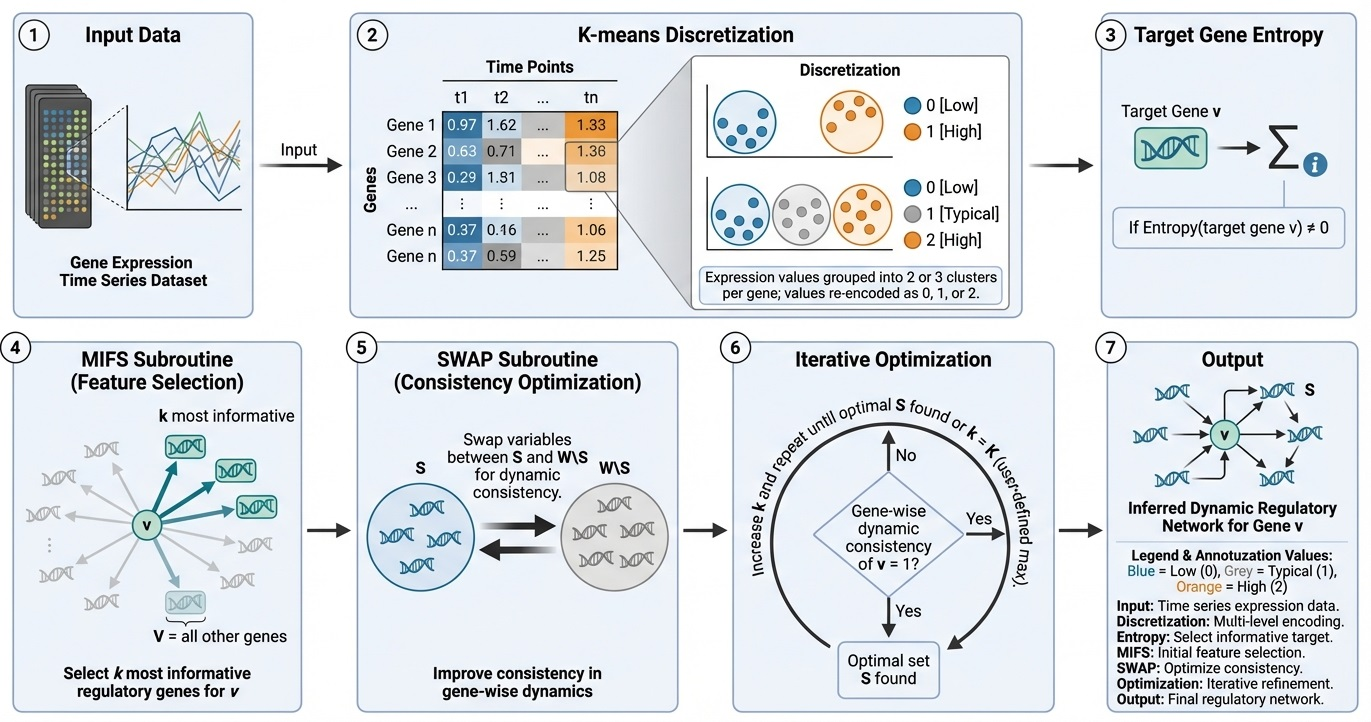
\includegraphics[width=\linewidth]{Figures/chapter2_framework.png}
\decoRule
\caption{The overall framework of the MIDNI algorithm begins with a real-valued time-series gene expression dataset, which is transformed into a discretized expression dataset through the K-means discretization algorithm. The number of clusters \( K \) for each gene is adaptively determined using a validity index, ensuring that the discretization captures the inherent distribution of the gene's expression values. The discretized dataset is subsequently processed by the \textbf{MIFS} and \textbf{SWAP} subroutines, which identify the most informative regulatory genes for each target gene. The output of these subroutines is a collection of candidate regulatory sets for all genes in the network. Using these results, the gene regulatory network is reconstructed into a predictive network that can model and simulate the dynamic interactions among genes.}
\label{fig:chapter2_framework}
\end{figure}

\subsubsection{Discretization}

Boolean discretization can significantly accelerate the network inference process, and it is well-suited for a subset of genes whose expression dynamics are sufficiently captured by two discrete states. Nevertheless, other genes exhibit more complex expression patterns that are better represented using a higher-level discretization, as illustrated in Figure~\ref{fig:chapter2_discretization}. Indeed, previous studies have demonstrated the advantage of employing three-level discretization for gene expression data. For instance, Deep Neural Network approaches \parencite{Ahn2019} utilize the values $1$, $0$, and $-1$ to quantify individual gene contributions, reflecting upregulated, unchanged, and downregulated states. Similarly, several other methods \parencite{Ji2004,Madeira2005, Gallo2013} have adopted a ternary discretization scheme for genes, where $1$, $0$, and $-1$ correspond to \enquote{upregulated}, \enquote{no-change}, and \enquote{downregulated}, providing a more nuanced representation of gene activity that captures intermediate regulatory effects.

Therefore, MIDNI adopts a hybrid discretization strategy, utilizing both binary (two-level) and ternary (three-level) representations. To select the optimal discretization level for each gene, the validity index is employed \parencite{Ray1999, Halkidi2001, Shen2005}, which provides a quantitative measure of the clustering quality and is defined as follows:

\begin{equation}
\text{Validity} = \frac{\text{Intra}}{\text{Inter}},
\end{equation}

where

\begin{equation}
\text{Intra} = \frac{1}{P} \sum_{i=1}^{k} \sum_{x \in C_i} \lVert x - z_i \rVert^2,
\end{equation}

and

\begin{equation}
\text{Inter} = \min_{i,j} \lVert z_i - z_j \rVert^2,
\quad i \neq j \in \{1,2,\ldots,k\},
\end{equation}
where \( P \) represents the total number of observed time points for the gene, \( k \) is the number of clusters, and \( z_i \) denotes the centroid of cluster \( C_i \). The optimal number of clusters is then determined by selecting the value of \( k \) that minimizes the validity index, thereby ensuring an appropriate balance between cluster compactness and separation.

\begin{figure}[th]
\centering
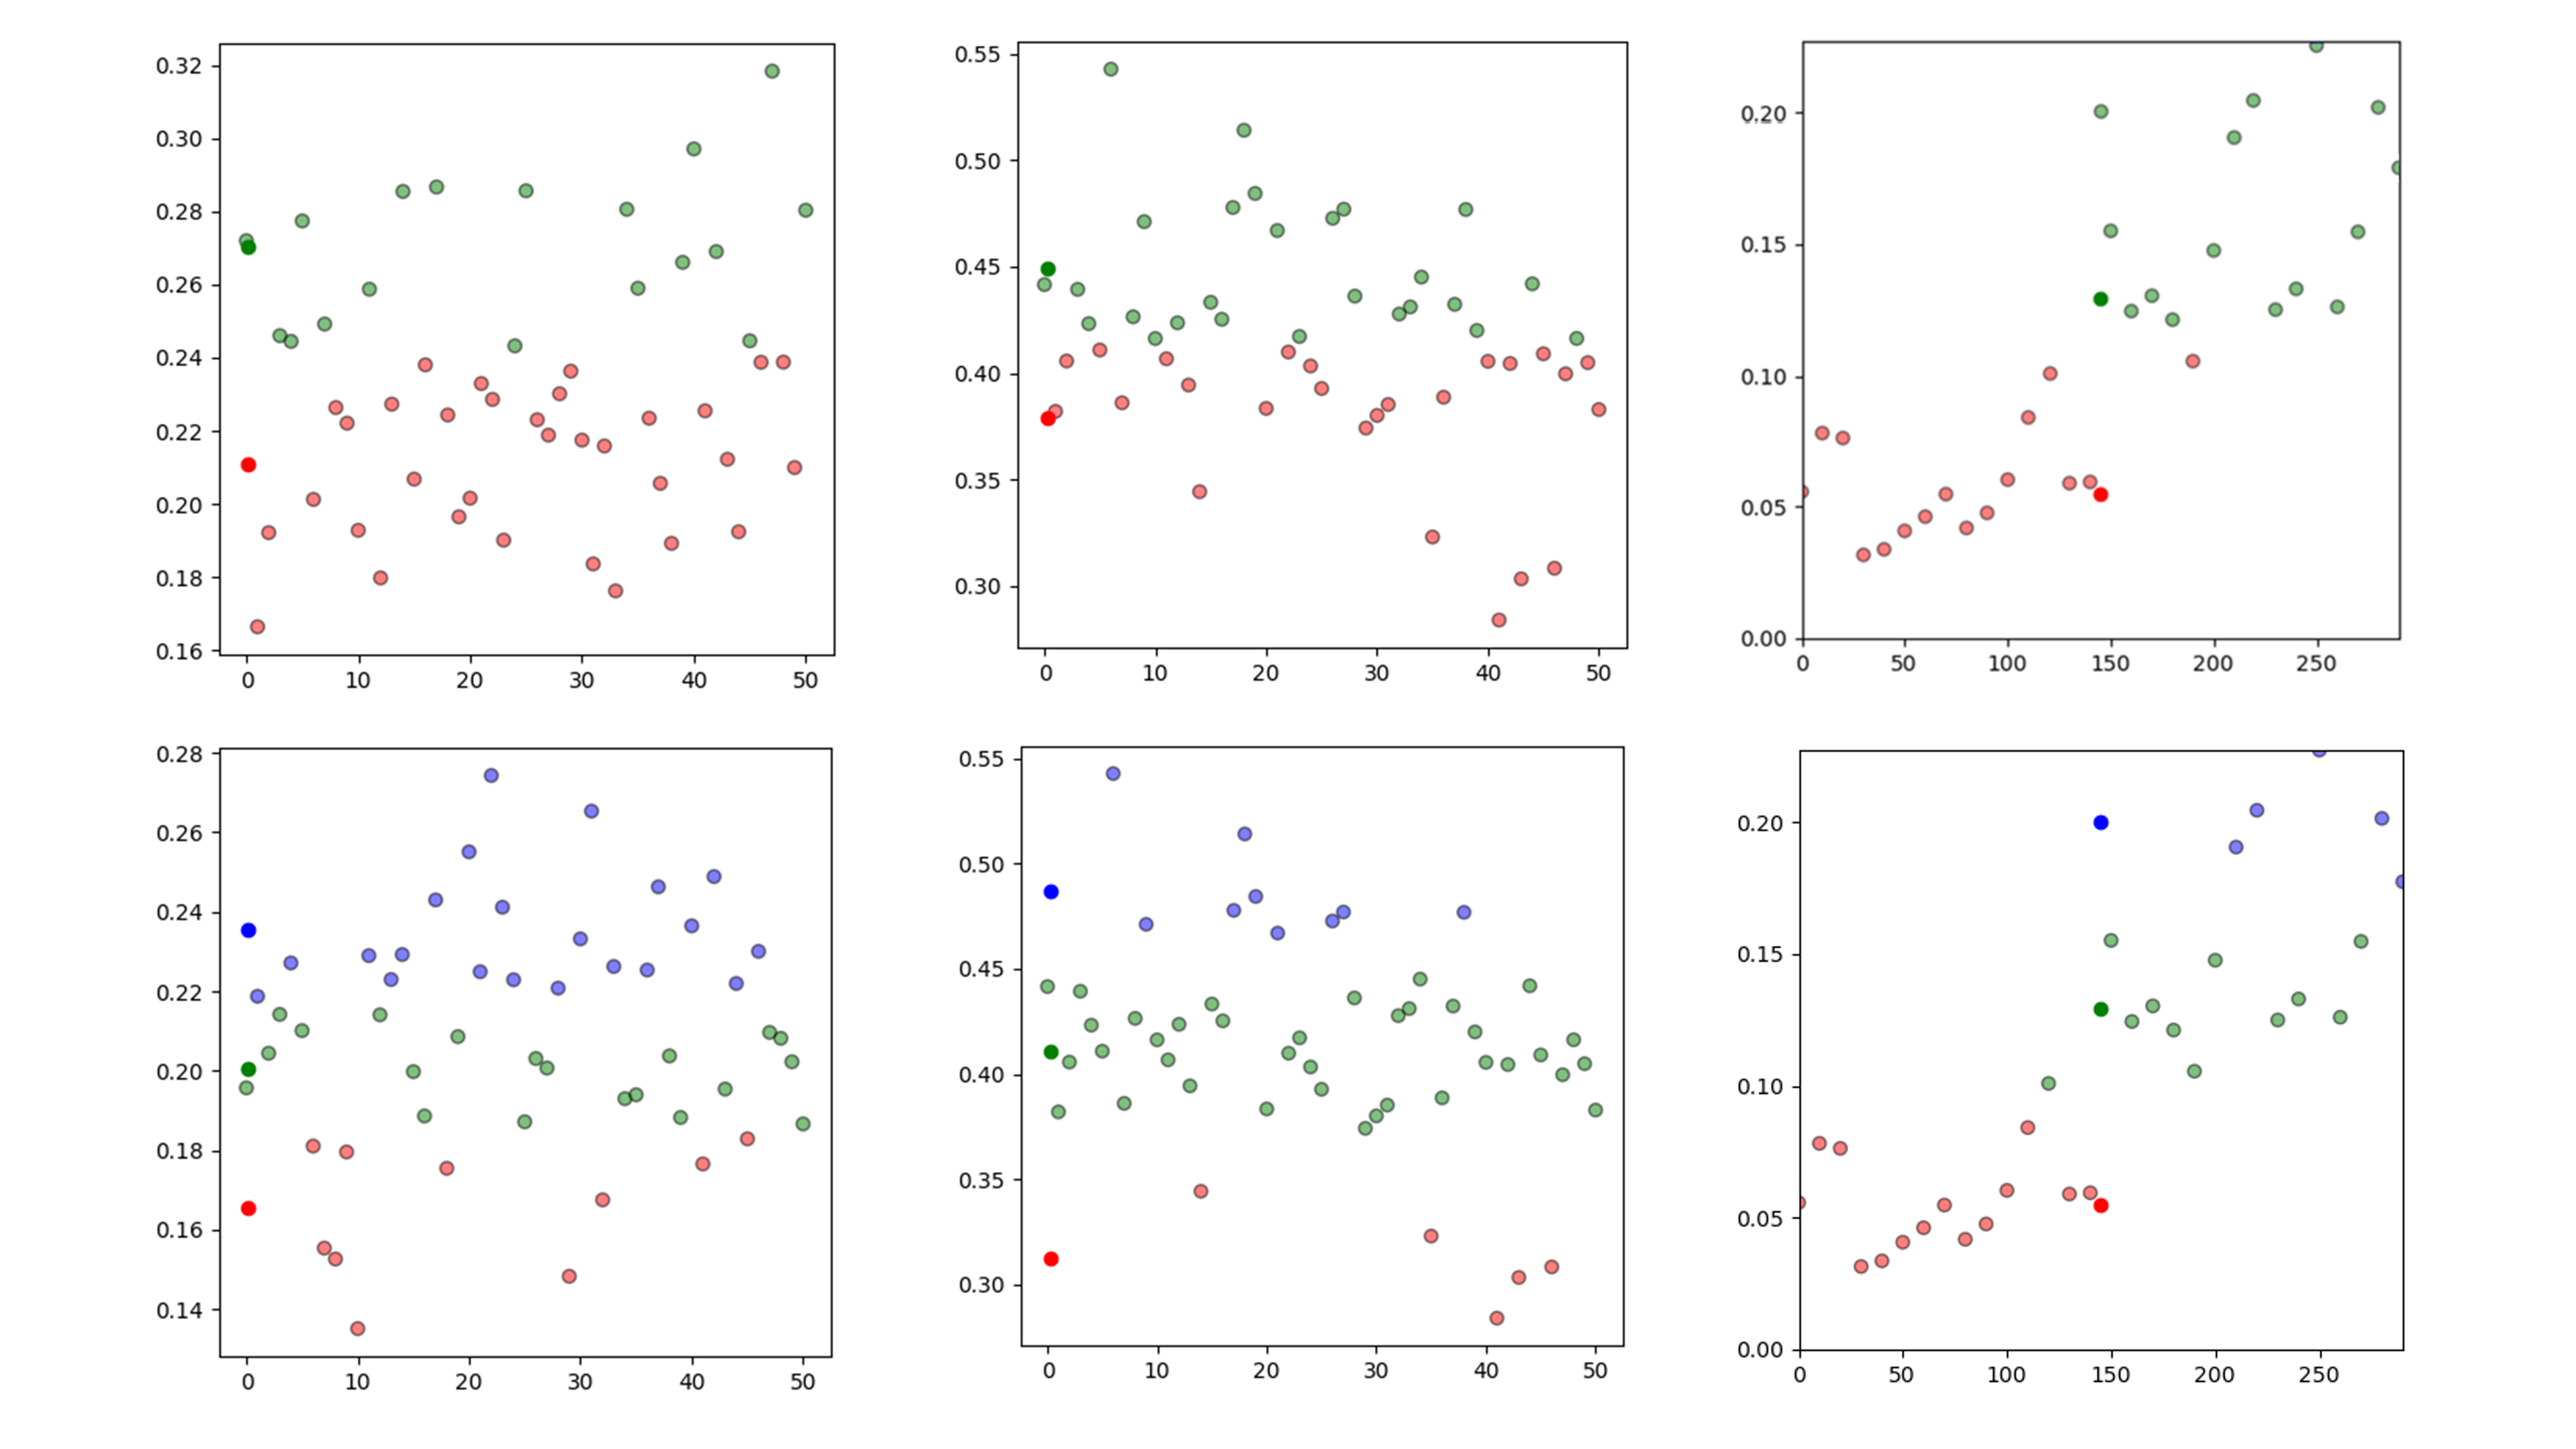
\includegraphics[width=\linewidth]{Figures/chapter2_discretization.png}
\decoRule
\caption{Illustrative examples of discretization for three different genes under two discretization scenarios. 
The upper row shows the discretized expression profiles obtained with $k = 2$, while the lower row presents the corresponding results with $k = 3$. 
For each gene, the x-axis represents the time points and the y-axis denotes the real-valued gene expression levels prior to discretization, highlighting how different discretization levels capture distinct expression patterns.}
\label{fig:chapter2_discretization}
\end{figure}
More specifically, each gene is discretized using K-means clustering with both two-class and three-class configurations.  
For each discretization scheme, the corresponding validity index is computed.  
The gene is then assigned to the discretization level (two or three classes) that yields the smaller validity index, indicating a better clustering structure.  
This procedure is applied independently to all genes in the network.

\subsubsection{MIFS and SWAP subroutines}

Given a discretized time-series gene expression dataset, \textit{MIDNI} executes two subroutines, \textit{MIFS} and \textit{SWAP}, in sequence.  
We note that these subroutines were adapted from those of \textit{MIBNI}~\parencite{Barman2017}, since the original versions were designed exclusively for binary-valued gene expression data.

For each target gene $v$ in the network, the \textit{MIFS} subroutine identifies an initial subset of regulatory candidates $S_v \subseteq V$ by evaluating an approximation of multivariate mutual information (see Algorithm~\ref{fig:chapter2_mifs}).  
Afterward, the \textit{SWAP} subroutine (see Algorithm~\ref{fig:chapter2_swap}) iteratively searches for an improved regulatory set beginning from $S_v$.

The function \texttt{search\_update\_rule} is responsible for identifying a set of update rules in the update table such that the regulatory set $S_v$ can perfectly reproduce the discretized trajectory of the target gene $v$.  
An illustrative example of the \texttt{search\_update\_rule} function is provided in the Appendix.

More specifically, the \textit{SWAP} procedure repeatedly tests pairwise swaps between candidate regulatory genes in $S_v$ (denoted as $S$ in Algorithm~\ref{fig:chapter2_swap}) and genes in the complement set $V \setminus S_v$ (denoted as $W$).  
These swaps are tested exhaustively for all gene pairs across the two sets, following a decreasing order of mutual information with respect to the target gene.  

As a final output, \textit{MIDNI} produces the optimal regulatory gene set identified for each target gene in the network.
\begin{figure}[th]
\centering
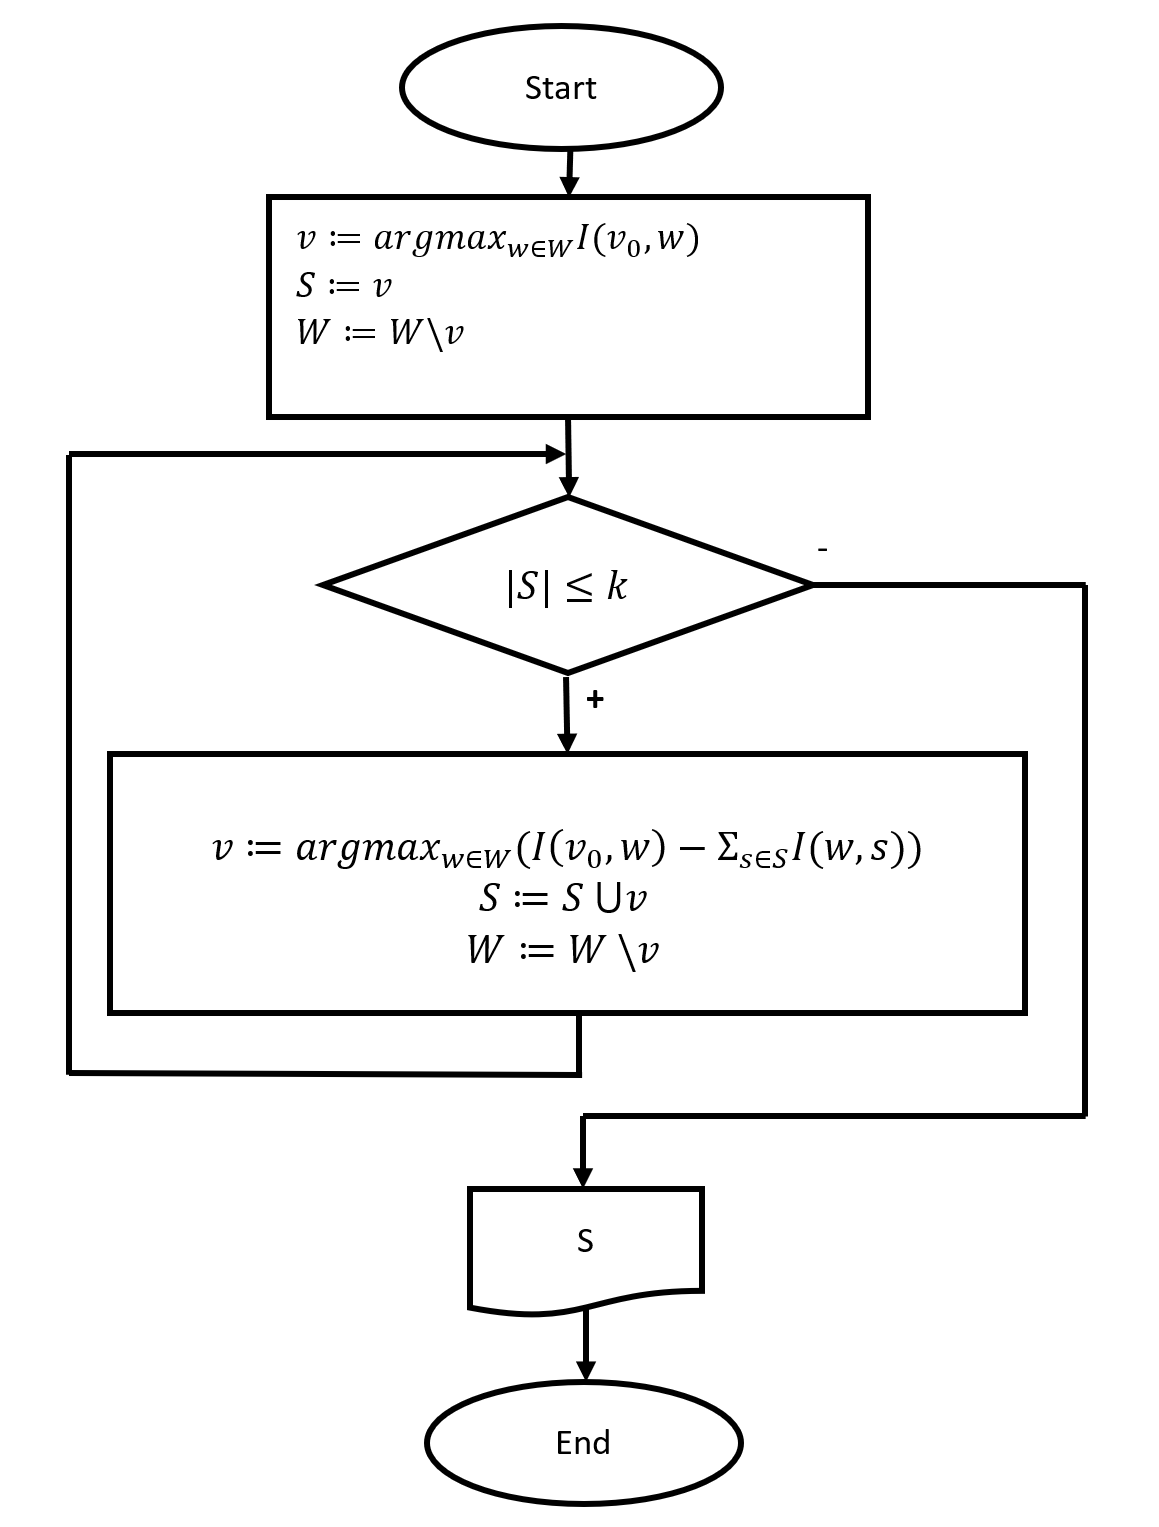
\includegraphics[width=\linewidth]{Figures/chapter2_mifs.png}
\decoRule
\caption{The subroutine \textit{MIFS}$(v_0, W, k)$, where $v_0$ is the target variable, 
$W = \{w_1, w_2, \ldots, w_M\}$ is the set of variables, 
and $k$ is the desired number of input variables.}
\label{fig:chapter2_mifs}
\end{figure}

\begin{figure}[th]
\centering
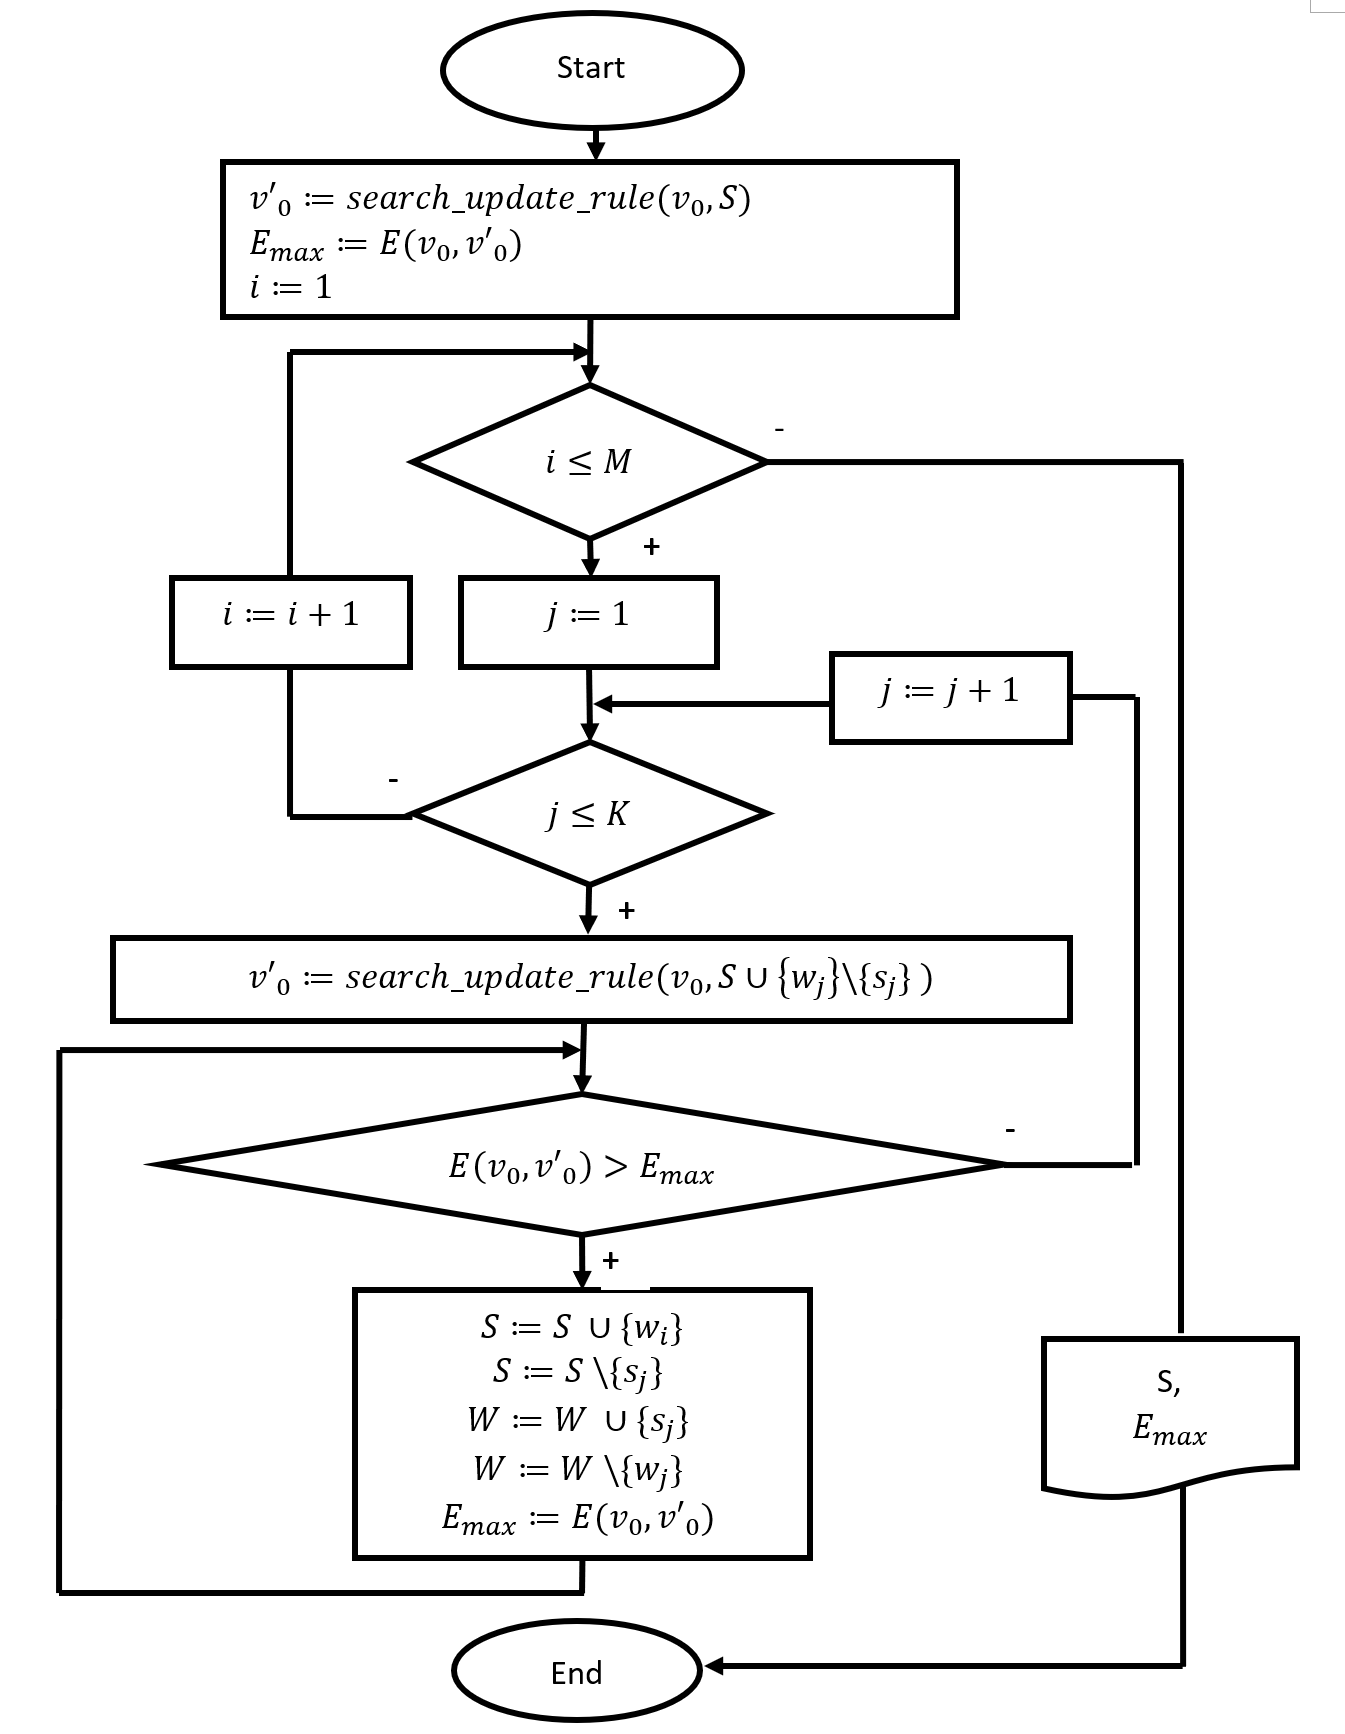
\includegraphics[width=\linewidth]{Figures/chapter2_swap.png}
\decoRule
\caption{The subroutine \textit{SWAP}$(v_0, S, W)$, where $v_0$ is the target variable; 
$S = \{s_1, s_2, \ldots, s_k\}$ is the set of selected variables such that 
$I(v_0, s_i) \geq I(v_0, s_j)$ if $i < j$ for all $s_i, s_j \in S$; 
and $W = \{w_1, w_2, \ldots, w_M\}$ is the set of unselected variables such that 
$I(v_0, w_i) \geq I(v_0, w_j)$ if $i < j$ for all $w_i, w_j \in W$.}
\label{fig:chapter2_swap}
\end{figure}

\section{Experiments, Results, and Discussions}\label{chapter2_result}
\subsection{Experiments}The whole process can be divided into three main stages.  
In the first stage, the input gene expression data are discretized using the K-means clustering algorithm.  
The resulting discretized dataset is then processed by the \textit{MIDNI} framework, whose output is a predicted regulatory structure of the underlying gene network. In the final stage, this inferred structure is evaluated by comparing it with the ground-truth network using tools that measure both structural and dynamical accuracies. All stages of the workflow are implemented using the Python programming language and its scientific libraries. To assess the performance and robustness of \textit{MIDNI}, we conducted experiments on two types of time-series gene expression datasets: an artificial discretized dataset and a real-valued dataset generated from Hill-function–based simulations. 

\subsection{Results} \label{sec:results}
\noindent\textbf{Case study 1: Artificial discretized dataset}\par
We generated an artificial dataset consisting of 20 groups of discretized networks with sizes 
$|V| = 10, 20, \ldots, 190, 200$.  
Each group contains 20 independently generated random networks, resulting in a total of 400 networks used in this simulation study.  
For each target gene, the regulatory structure was created by randomly selecting $k$ regulators from all genes except the target gene itself.  
The value of $k$ was also sampled uniformly at random from the interval $[1, \text{maximum number of regulators allowed}]$ for each target gene (see Table~\ref{tab:dataset_parameters}).

\begin{table}[htbp]
\centering
\caption{The settings used for generating the datasets.}
\begin{tabular}{lcc}
\hline
\textbf{Parameters} & \textbf{Discretized dataset} & \textbf{Real-valued dataset} \\
\hline
Size of networks ($N$) & 10, 20, ..., 190, 200 & 50, 100, 200, 300 \\
Noise rate & None & 0, 5, 10 \\
Time lag & 1 & 1 \\
Number of observed time points & 30 & 30 \\
Number of regulators in the network & $0.4 \times N$ & $0.4 \times N$ \\
Maximum regulators for each gene & 4--8 & 4--8 \\
Max expression ($\alpha_{\text{max}}$) & NA & 0.1--1 \\
Basal expression ($\beta_0$) & NA & 0.1--1 \\
Apparent dissociation constant ($K_d$) & NA & 1--5 \\
Hill coefficient ($n$) & NA & 1--5 \\
\hline
\end{tabular}
\label{tab:dataset_parameters}
\end{table}
In this simulation setting, the initial state of each gene was randomly assigned one of the three discrete values 0, 1, or 2. The state of every node was then updated across 29 consecutive time-steps using a discrete update function, which was chosen uniformly at random from the full set of possible functions. For a target gene regulated by \( k \) genes, the number of possible update functions is \( 3^{(3^k)} \). Based on this procedure, we generated the artificial discretized time-series dataset without requiring any additional discretization step (the detailed parameter configuration is summarized in Table~\ref{tab:dataset_parameters}).

The inference results obtained by MIDNI are shown in Figure~\ref{fig:chapter2_case1_dynamics_performance}. As illustrated, the dynamics accuracy was close to 1.0 across all network sizes. This near-perfect performance is likely related to the constraint that each gene has at most eight regulatory inputs. Regarding structural metrics, precision and recall gradually decreased as the network size increased, whereas the structural accuracy increased. The latter trend is expected because larger networks contain more candidate non-regulatory pairs, leading to an increase in true negative cases.

To further assess the robustness of MIDNI, we evaluated how the number of incoming regulatory links (\( D \)) affects inference quality (Figure~\ref{fig:chapter2_case1_incoming_links}). In the gold-standard networks, \( D \) represents the true number of regulators for a given target gene and reflects the intrinsic difficulty of the inference task. The generated networks exhibited \( D \in [1, 8] \). When \( D = 1 \) or \( D = 2 \), all performance indicators—both dynamics and structure-based—were nearly perfect. For \( D > 2 \), the structural metrics progressively declined, although the dynamics accuracy remained close to 1.0 even at \( D = 8 \).

These observations highlight the multimodal nature of the GRN inference problem: many different network structures can produce nearly identical dynamical behaviors. Consequently, MIDNI consistently identifies networks that replicate the temporal dynamics of the gold-standard networks, whereas perfect structural recovery becomes inherently challenging due to this multimodality.

\begin{figure}[!th]
\centering
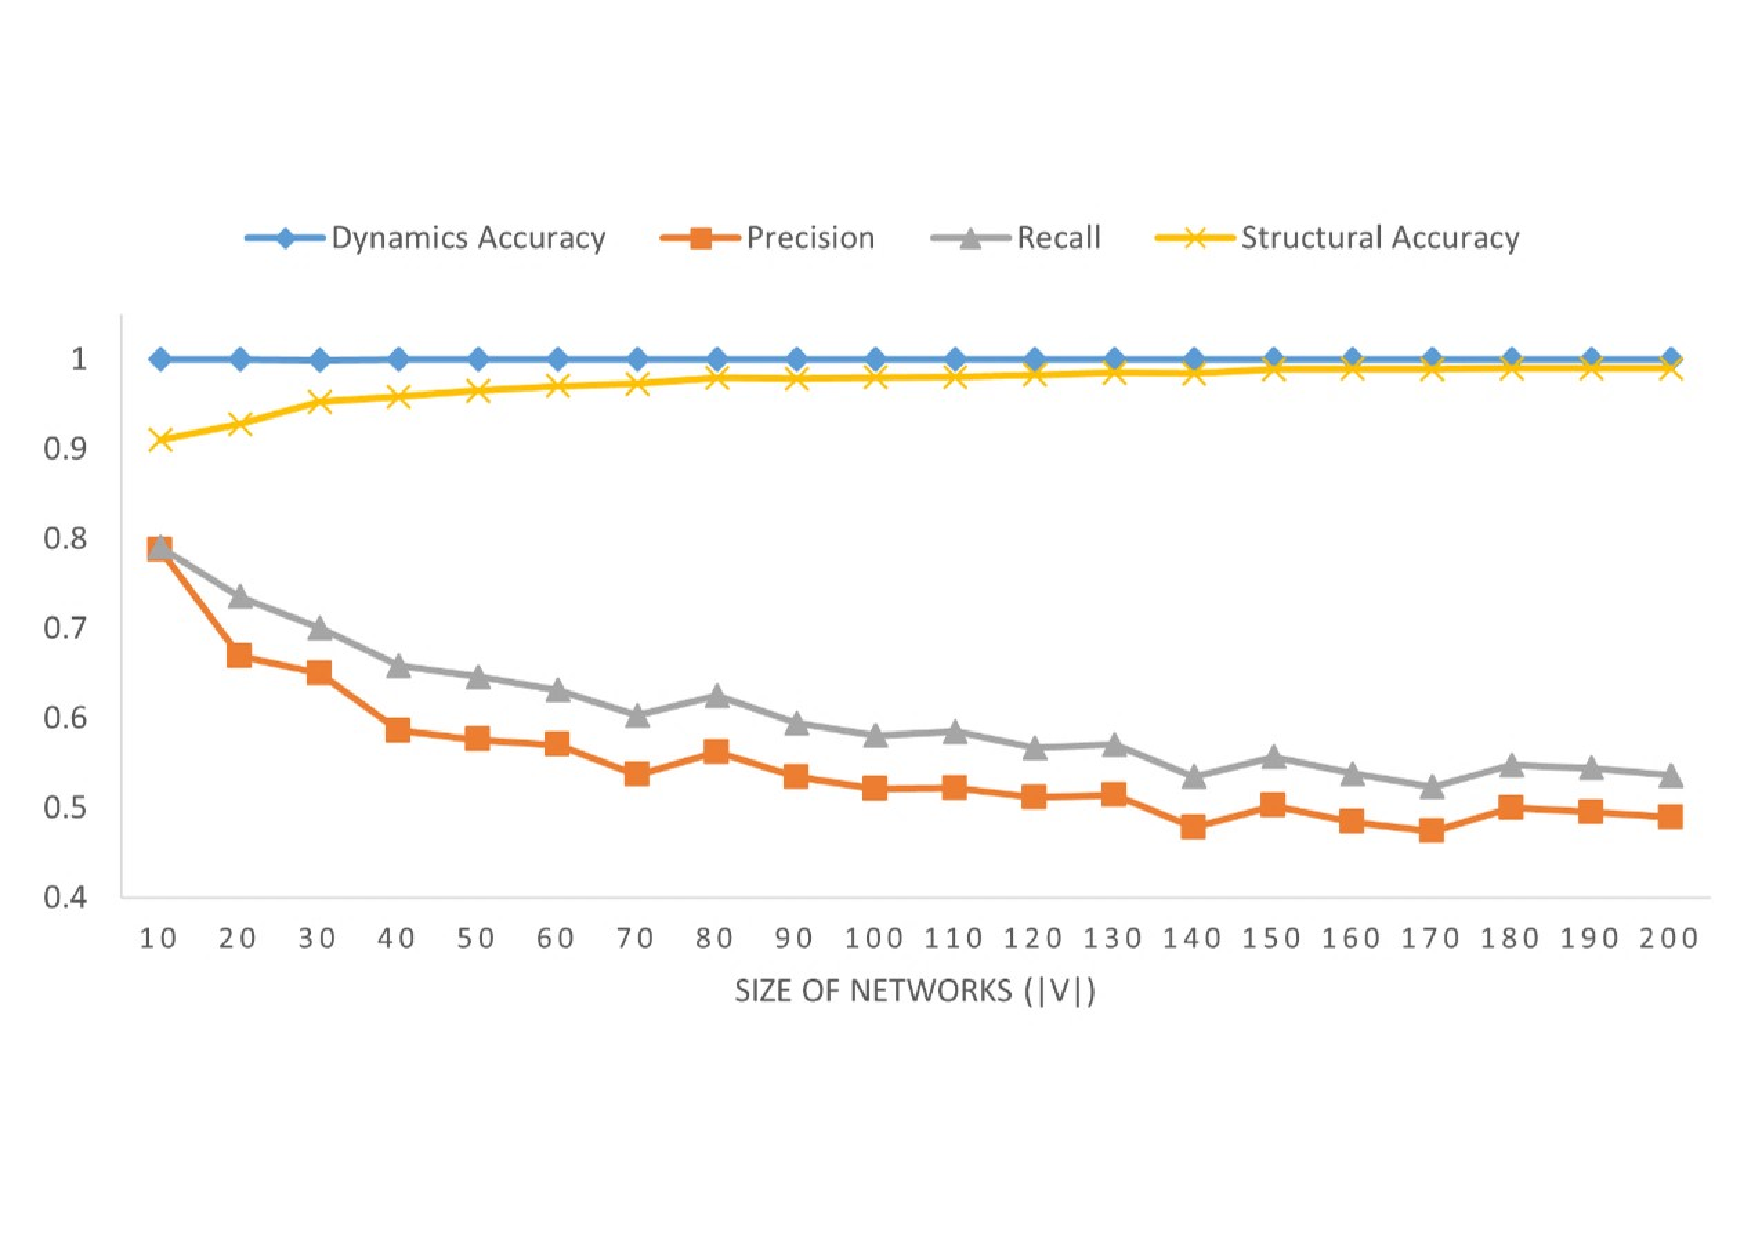
\includegraphics[width=\linewidth]{Figures/chapter2_case1_dynamics_performance.pdf}
\decoRule
\caption[]{The performance of MIDNI on the artificial discretized dataset. The x-axis means the network size denoted by the number of genes in the network. For each size, the y-axis shows the average value of each performance metric over 20 random networks.}
\label{fig:chapter2_case1_dynamics_performance}
\end{figure}

\begin{figure}[th]
\centering
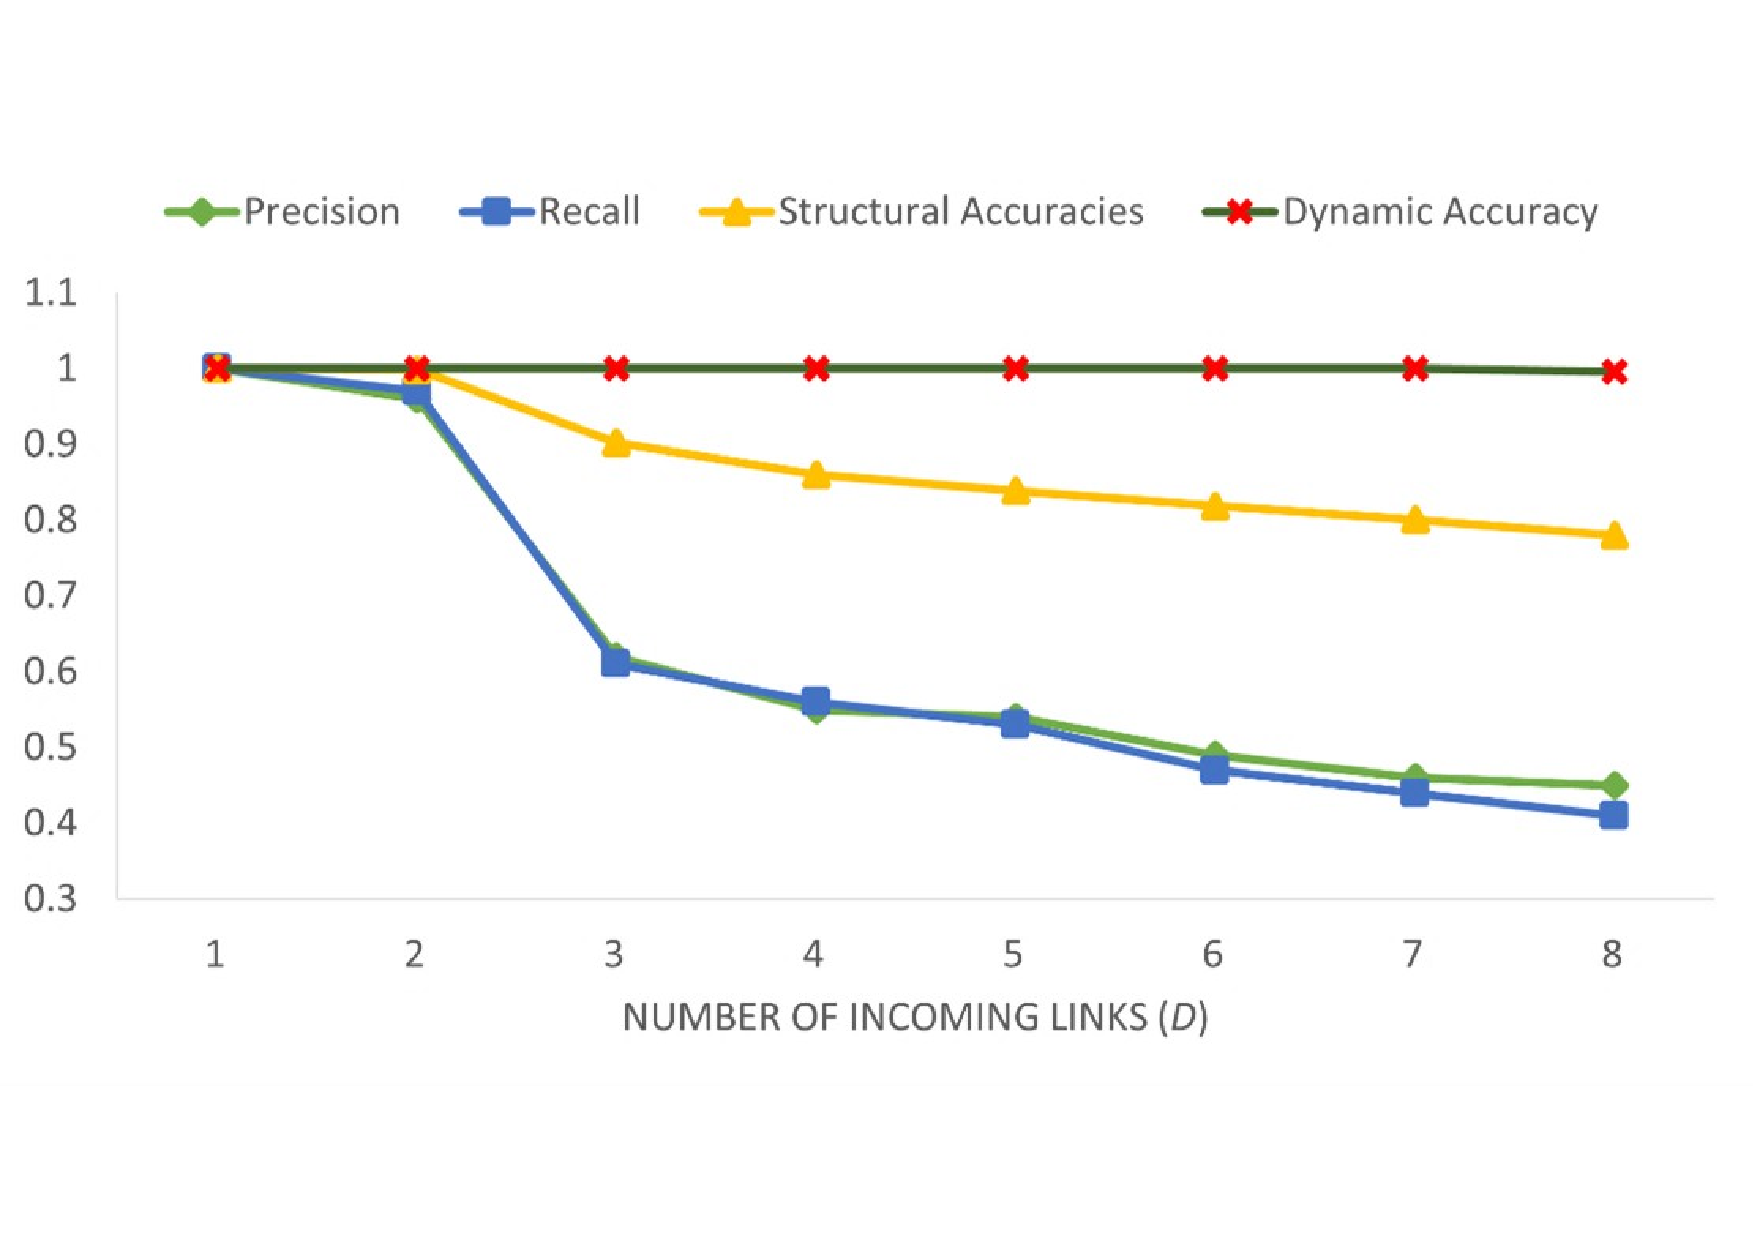
\includegraphics[width=\linewidth]{Figures/chapter2_case1_incoming_links.pdf}
\decoRule
\caption{Inference performance according to the number of incoming links (\textit{D}) in the gold-standard network.}
\label{fig:chapter2_case1_incoming_links}
\end{figure}
\noindent\textbf{Case study 2: Artificial real-valued dataset}\par

MIDNI was further evaluated using a real-valued time-series gene expression dataset generated based on the Hill function \parencite{Santillan2008}. This dataset contains four groups of networks with sizes $|V| = 50, 100, 200,$ and $300$. Each group includes 20 independently generated random networks, resulting in a total of 80 networks for this experiment. The procedure for constructing the network topology followed the same approach used for the artificial discretized dataset. The Hill function employed to simulate the continuous gene expression dynamics is given below, and its corresponding parameter settings are summarized in Table~\ref{tab:dataset_parameters}.

\[
[\text{Protein}] =
\begin{cases}
\alpha_{\max} \left( \beta_0 + (1 - \beta_0)\dfrac{[\text{TF}]^n}{K_d + [\text{TF}]^n} \right), & \text{for activation}, \\[10pt]
\alpha_{\max} \left( \beta_0 + (1 - \beta_0)\dfrac{K_d}{K_d + [\text{TF}]^n} \right), & \text{for inhibition},
\end{cases}
\]

where $\alpha_{\max}$, $\beta_0$, TF, $K_d$, and $n$ represent the maximum transcriptional output, the basal expression level, the transcription factors regulating the gene, the apparent dissociation constant, and the Hill coefficient, respectively. As described in Section~3.2.1, the expression profile of each gene was discretized using K-means clustering, where the number of clusters $k$ was chosen to be either two or three depending on the underlying distribution of the gene’s expression values.

We first assessed the proportion of genes assigned to the three-level discretization category, as illustrated in Figure~\ref{fig:chapter2_propotion}. Except for the networks of size 10, the proportions of genes discretized into two levels and those discretized into three levels were approximately balanced. This observation indicates that ternary discretization occurs as frequently as binary discretization within our framework.

To further evaluate performance, we compared MIDNI against several representative inference algorithms—DBN, MICRAT, MIBNI, and GENIE3—using artificial time-series gene expression datasets. DBN \parencite{Zou2005} identifies potential regulators by analyzing the earliest time points at which gene expression exhibits up- or down-regulation. MICRAT \parencite{Yang2018} constructs an undirected association graph based on the maximal information coefficient, and subsequently assigns edge directions using average entropy. GENIE3 \parencite{HuynhThu2010}, a tree-based inference approach, was the top-performing method in the DREAM4 In Silico Multifactorial Challenge. MIBNI represents our earlier Boolean-based method for network reconstruction.

\begin{figure}[th]
\centering
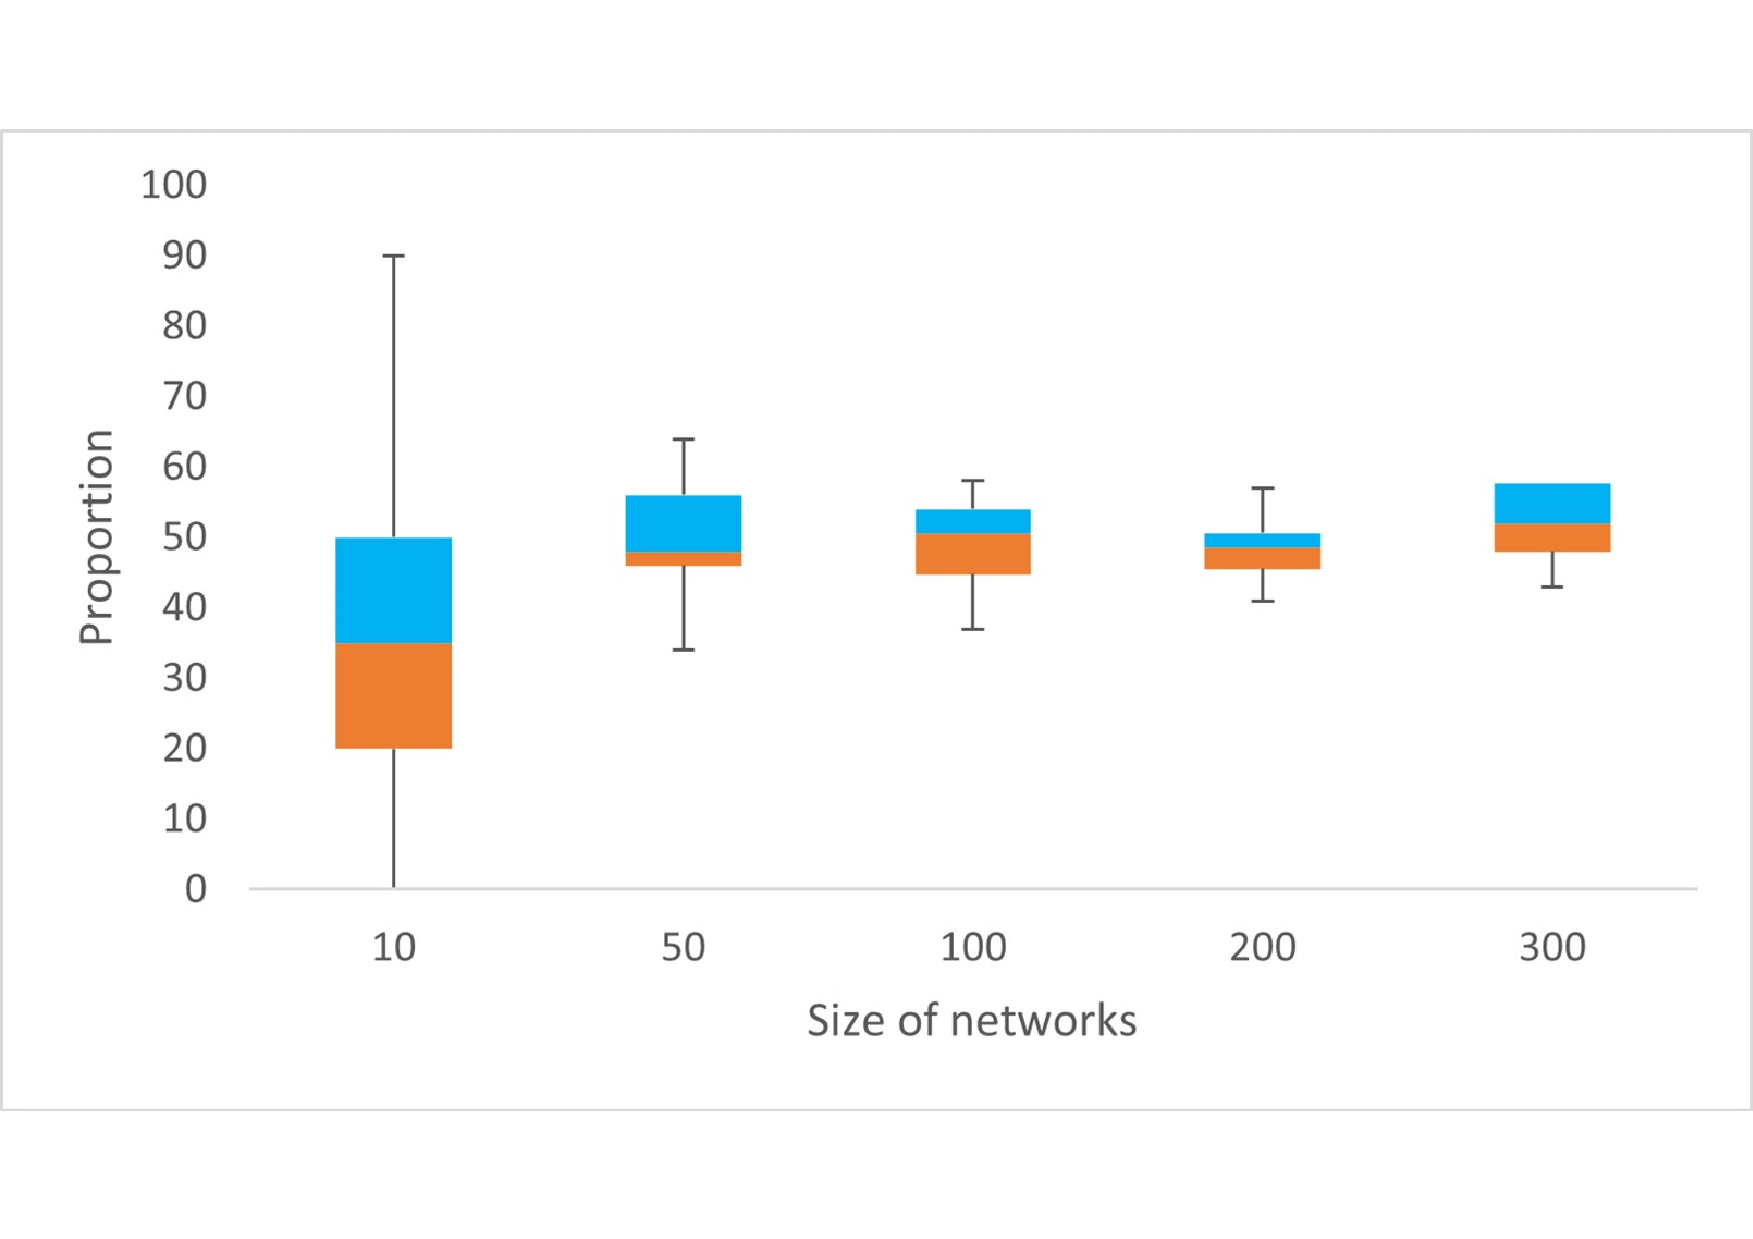
\includegraphics[width=\linewidth]{Figures/chapter2_propotion.pdf}
\decoRule
\caption{The proportion of three-level discretized genes in the networks.}
\label{fig:chapter2_propotion}
\end{figure}
\par
\vspace{1em}
\noindent\textbf{Structural accuracy analysis}\par
\vspace{0.5em}
We grouped all target genes into eight categories based on the number of incoming regulatory links ($D$), which varies from 1 to 8, as illustrated in Figure~\ref{fig:chapter2_structure_accuracy}. As shown in the figure, the structural accuracy of all inference methods consistently declined as $D$ increased. 
This trend occurs because a larger number of incoming links makes the inference task inherently more challenging. When $D = 1$, nearly all methods successfully identified the optimal solution. However, as $D$ grew, their performance decreased in an approximately linear manner.

We emphasize that our proposed method achieved the highest structural accuracy in every setting, except for the cases $D = 1$ and $D = 2$ in the smallest network ($|V| = 50$). The performance advantage became more pronounced when both the network size and the value of $D$ were large. These findings demonstrate the effectiveness of our approach in large-scale and complex inference scenarios. Furthermore, the integration of multi-level discretization provided additional improvement compared with our previous method, MIBNI.

\begin{figure}[th]
\centering
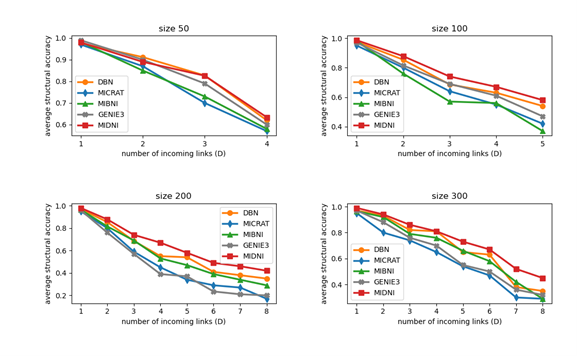
\includegraphics[width=\linewidth]{Figures/chapter2_structure_accuracy.png}
\decoRule
\caption{Structural performance on random real-valued networks. Four network size groups ($|V| = 50, 100, 200, 300$) were examined, with 20 randomly generated networks for each size. Target genes were categorized based on the number of incoming regulatory links ($D$) in the gold-standard network. The x-axis represents the values of $D$, while the y-axis indicates the average structural accuracy across networks.}
\label{fig:chapter2_structure_accuracy}
\end{figure}
\par
\vspace{1em}
\noindent\textbf{Dynamics accuracy analysis}\par
\vspace{0.5em}
We recognize that distinct network structures can sometimes lead to the same underlying dynamics. 
Therefore, it is also important to evaluate the inference performance in terms of dynamics accuracy. 
We assessed the dynamics accuracies of the inferred networks generated by MIDNI, DBN, MICRAT, MIBNI, 
and GENIE3. Similar to the structural accuracy analysis, we examined how the number of regulatory 
genes for each target gene ($D$) influences the dynamics accuracy of each method. The corresponding 
results are presented in Figure~\ref{fig:chapter2_dynamic_accuracy}. 

As shown in the figure, most methods achieved dynamics accuracy close to 1.0 when $D = 1$. 
As $D$ increases, the inference task becomes more challenging, resulting in lower dynamics accuracies. 
However, MIDNI exhibited the best performance in all cases except for $D = 3$ in the network group 
with size $|V| = 300$. In particular, for $D = 8$ in the network groups of sizes 200 and 300, 
MIDNI achieved a dynamics accuracy of approximately 0.6, while the other methods remained around 0.5. 
These results highlight the strong inference capability of our method for more complex and larger-scale networks.

\begin{figure}[th]
\centering
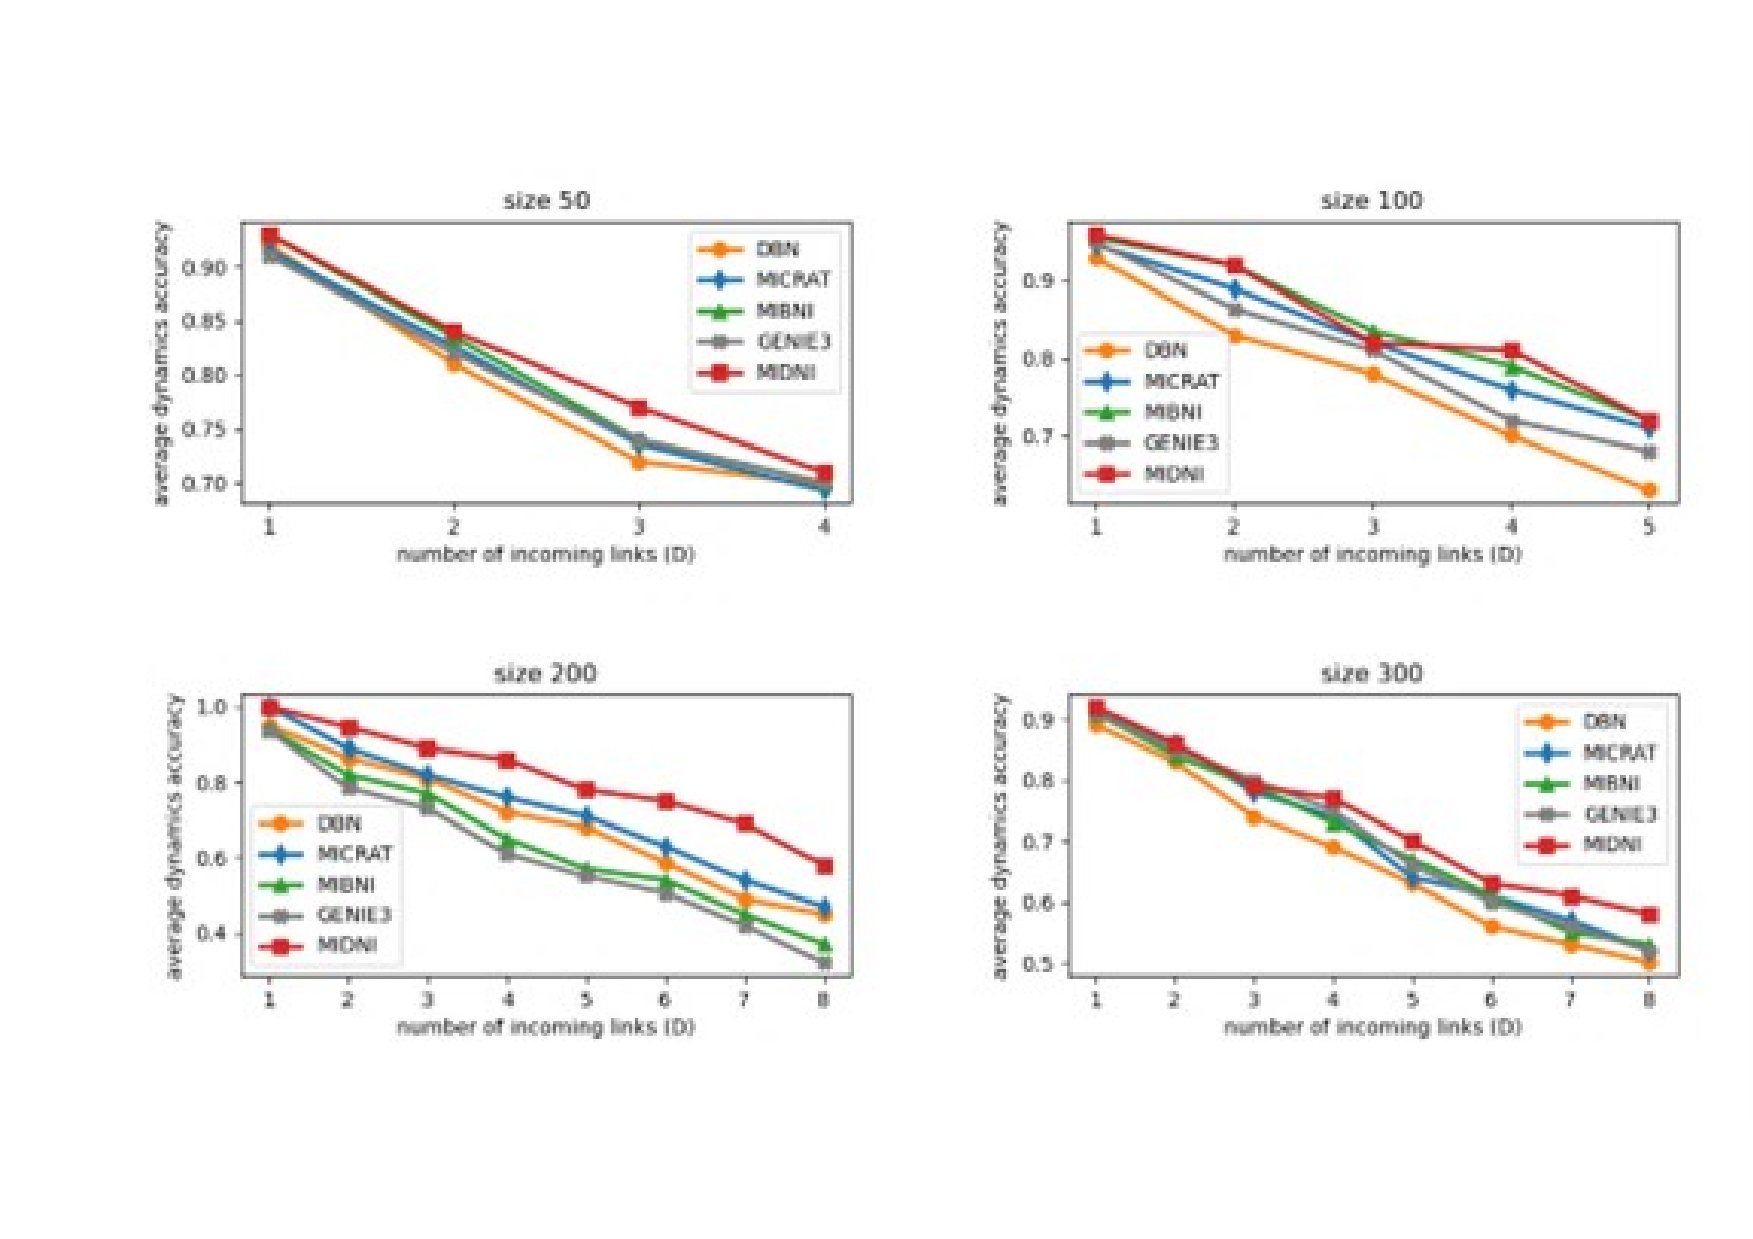
\includegraphics[width=\linewidth]{Figures/chapter2_dynamic_accuracy.pdf}
\decoRule
\caption{Dynamical performance on the random real-valued networks. Four size groups of networks ($|V| = 50, 100, 200, \text{ and } 300$) were considered, and 20 random networks were generated for each group. All target genes are grouped according to the number of incoming links ($D$) in the gold-standard network, and the x-axis represents the $D$ values. The y-axis shows the average dynamics accuracy.}
\label{fig:chapter2_dynamic_accuracy}
\end{figure}
\vspace{1em}
\noindent\textbf{Running time}\par
\vspace{0.5em}
To assess the computational efficiency of MIDNI in comparison with other inference methods, 
we evaluated the average running time over the 80 random networks described in Case Study~2. 
All experiments were performed on a PC equipped with an AMD Ryzen 5 3400G 3.70~GHz CPU and 
16~GB RAM. The results are illustrated in Figure~\ref{fig:chapter2_running_time}, where the 
y-axis indicates the average running time in milliseconds for the four different network sizes.

Although MIDNI was noticeably slower than DBN and MICRAT, its running time was comparable 
to that of GENIE3 and MIBNI, and it was slightly faster than MIBNI. This improvement is due to 
several optimizations applied to the MIFS and SWAP subroutines in MIDNI compared to the original 
implementation. For instance, we employed built-in libraries such as \texttt{sklearn} and 
\texttt{scipy} to compute mutual information and entropy metrics, which are more efficient than 
custom-coded versions. We also utilized vectorized computations, which execute significantly 
faster than traditional for-loop based calculations.

Considering that MIDNI achieved superior structural and dynamics inference accuracy compared 
with the other methods, it is a desirable choice when high accuracy is required, even at the 
expense of additional computational time.

\begin{figure}[th]
\centering
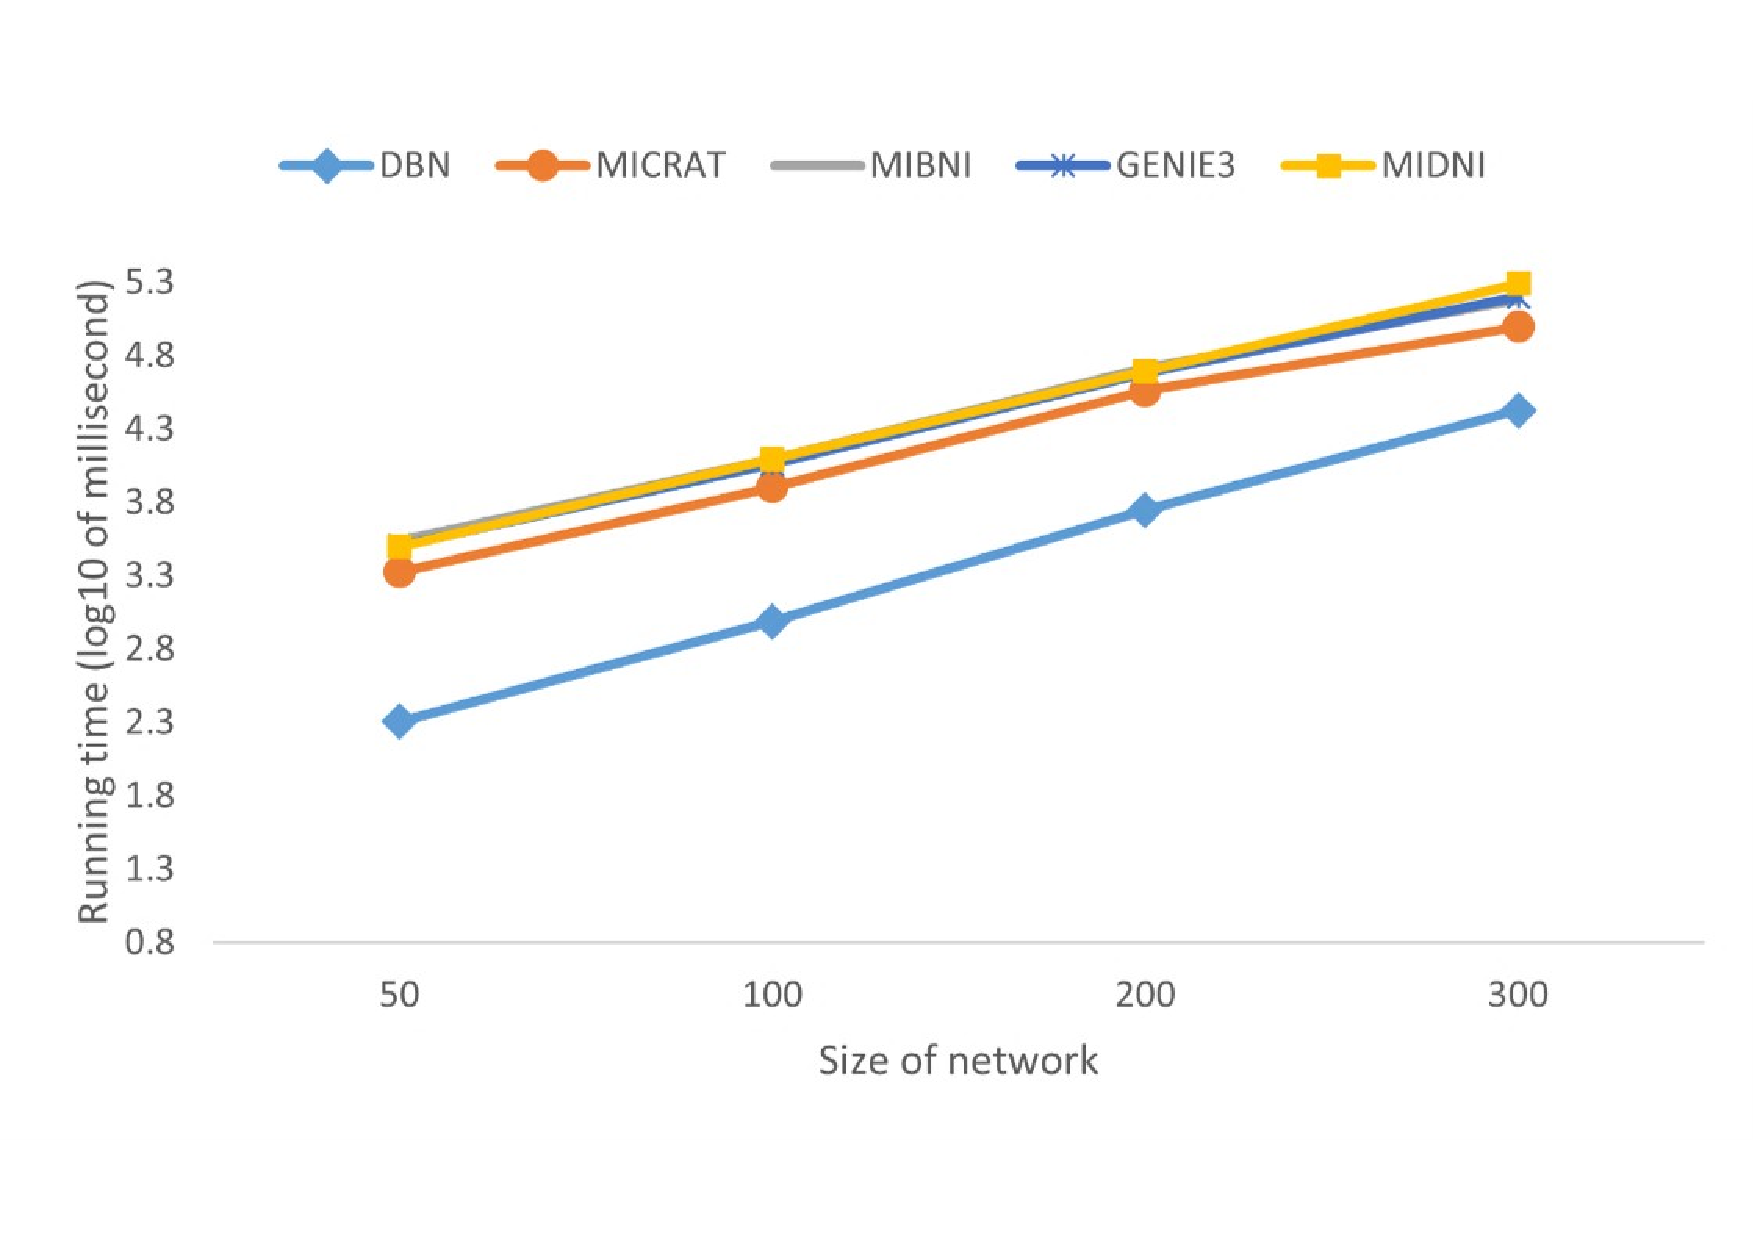
\includegraphics[width=\linewidth]{Figures/chapter2_running_time.pdf}
\decoRule
\caption{Comparison of running time across different network sizes. The x-axis represents the network size, while the y-axis shows the running time in milliseconds on a $\log_{10}$ scale.}
\label{fig:chapter2_running_time}
\end{figure}
\subsection{Discussions}
In this study, we proposed a new network inference method for time-series gene expression 
data, called MIDNI. The method first converts real-valued expression profiles into multi-level 
discretized values according to the underlying distribution of the expression data. Unlike 
most previous discretization-based inference approaches that employ Boolean network models, 
which may limit inference accuracy due to the oversimplified representation, MIDNI achieved 
superior performance in terms of both structural and dynamical accuracy, particularly in 
larger and more densely connected networks.

Despite these promising results, MIDNI has several limitations. First, the precision and recall 
values were not sufficiently high. We attribute this to the reliance on mutual information for 
selecting candidate regulatory genes that directly interact with a target gene. Some regulatory 
effects may be mediated through intermediate genes, which can lead to incorrect candidate 
selection. This suggests that integrating prior biological knowledge from existing databases 
may lead to more accurate predictions. Second, MIDNI uses the correlation coefficient to 
determine the interaction type and direction, which may also contribute to reduced accuracy. 
Finally, the MIFS and SWAP subroutines employed in MIDNI are greedy algorithms, and the inference 
performance could potentially be improved by incorporating more advanced or global search 
strategies.

\section{Conclusion \& Future Studies}\label{chapter2_conclusion}
\subsection{Conclusion}This study addresses one of the fundamental and challenging problems in computational 
biology, namely the inference of regulatory gene networks. The primary distinction of 
the proposed method compared with existing approaches lies in its use of a multi-level 
data representation scheme rather than relying on raw real-valued expression data or 
Boolean discretization. This choice not only prevents information loss during 
representation but also accelerates the inference process. Consequently, the method 
achieves superior structural and dynamical accuracy, particularly for large-scale 
networks.

Several key issues in network inference have been effectively addressed by the proposed 
approach:
\begin{itemize}
    \item \textbf{Adaptive discretization.} MIDNI determines the optimal number of clusters 
    (i.e., discretization levels) for each gene based on its expression value distribution.
    \item \textbf{Multivariate candidate evaluation.} The algorithm identifies plausible 
    regulatory genes using not only pairwise mutual information but also the approximate 
    dependency of a candidate on the set of previously selected regulators. This 
    multivariate assessment distinguishes MIDNI from most existing methods that consider 
    only pairwise interactions.
    \item \textbf{Enhanced structural and dynamical accuracy.} MIDNI improves not only the 
    structural agreement between inferred and gold-standard networks but also the 
    dynamical consistency of gene expression patterns within the network.
\end{itemize}

\subsection{Future Studies}
Although the proposed method outperformed other compared approaches, it still has 
several limitations, as discussed in subsection~\ref{sec:results}, which should be 
addressed in the next stage of this research. In the future, I plan to extend this 
study in several directions:
\begin{itemize}
    \item Develop a new subroutine capable of handling multimodal inference problems, 
    in which many optimal solutions may exist.
    \item Apply more sophisticated metrics to determine the direction of gene 
    interactions during inference, since the correlation coefficient is relatively 
    simple and may not sufficiently improve accuracy.
    \item Accelerate the inference process by integrating optimized search algorithms 
    or parallel computation techniques.
    \item Conduct experiments on data representation using alternative algorithms to 
    compare with the current K-means-based discretization.
    \item Attempt to infer networks using other types of data, such as steady-state 
    expression profiles (since this study used only time-series data), and incorporate 
    prior biological knowledge to further enhance inference accuracy.
\end{itemize}
